\PassOptionsToPackage{unicode=true}{hyperref} % options for packages loaded elsewhere
\PassOptionsToPackage{hyphens}{url}
%
\documentclass[10pt,xcolor=table,color={dvipsnames,usenames},ignorenonframetext,usepdftitle=false,french]{beamer}
\setbeamertemplate{caption}[numbered]
\setbeamertemplate{caption label separator}{: }
\setbeamercolor{caption name}{fg=normal text.fg}
\beamertemplatenavigationsymbolsempty
\usepackage{caption}
\captionsetup{skip=0pt,belowskip=0pt}
%\setlength\abovecaptionskip{-15pt}
\usepackage{lmodern}
\usepackage{amssymb,amsmath,mathtools,multirow}
\usepackage{float,hhline}
\usepackage{tikz}
\usepackage{mathtools}
\usepackage{ifxetex,ifluatex}
\usepackage{fixltx2e} % provides \textsubscript
\ifnum 0\ifxetex 1\fi\ifluatex 1\fi=0 % if pdftex
  \usepackage[T1]{fontenc}
  \usepackage[utf8]{inputenc}
  \usepackage{textcomp} % provides euro and other symbols
\else % if luatex or xelatex
  \usepackage{unicode-math}
  \defaultfontfeatures{Ligatures=TeX,Scale=MatchLowercase}
\fi
\usetheme[coding=utf8,language=french,
,titlepagelogo=img/logobeamer.png
]{TorinoTh}
% use upquote if available, for straight quotes in verbatim environments
\IfFileExists{upquote.sty}{\usepackage{upquote}}{}
% use microtype if available
\IfFileExists{microtype.sty}{%
\usepackage[]{microtype}
\UseMicrotypeSet[protrusion]{basicmath} % disable protrusion for tt fonts
}{}
\IfFileExists{parskip.sty}{%
\usepackage{parskip}
}{% else
\setlength{\parindent}{0pt}
\setlength{\parskip}{6pt plus 2pt minus 1pt}
}
\usepackage{hyperref}
\hypersetup{
            pdfauthor={Alain Quartier-la-Tente},
            pdfborder={0 0 0},
            breaklinks=true}
\urlstyle{same}  % don't use monospace font for urls
\newif\ifbibliography
\newlength{\cslhangindent}
\setlength{\cslhangindent}{1.5em}
\newlength{\csllabelwidth}
\setlength{\csllabelwidth}{3em}
\newenvironment{CSLReferences}[2] % #1 hanging-ident, #2 entry spacing
 {% don't indent paragraphs
  \setlength{\parindent}{0pt}
  % turn on hanging indent if param 1 is 1
  \ifodd #1 \everypar{\setlength{\hangindent}{\cslhangindent}}\ignorespaces\fi
  % set entry spacing
  \ifnum #2 > 0
  \setlength{\parskip}{#2\baselineskip}
  \fi
 }%
 {}
\usepackage{color}
\usepackage{fancyvrb}
\newcommand{\VerbBar}{|}
\newcommand{\VERB}{\Verb[commandchars=\\\{\}]}
\DefineVerbatimEnvironment{Highlighting}{Verbatim}{commandchars=\\\{\}}
% Add ',fontsize=\small' for more characters per line
\usepackage{framed}
\definecolor{shadecolor}{RGB}{248,248,248}
\newenvironment{Shaded}{\begin{snugshade}}{\end{snugshade}}
\newcommand{\AlertTok}[1]{\textcolor[rgb]{0.94,0.16,0.16}{#1}}
\newcommand{\AnnotationTok}[1]{\textcolor[rgb]{0.56,0.35,0.01}{\textbf{\textit{#1}}}}
\newcommand{\AttributeTok}[1]{\textcolor[rgb]{0.77,0.63,0.00}{#1}}
\newcommand{\BaseNTok}[1]{\textcolor[rgb]{0.00,0.00,0.81}{#1}}
\newcommand{\BuiltInTok}[1]{#1}
\newcommand{\CharTok}[1]{\textcolor[rgb]{0.31,0.60,0.02}{#1}}
\newcommand{\CommentTok}[1]{\textcolor[rgb]{0.56,0.35,0.01}{\textit{#1}}}
\newcommand{\CommentVarTok}[1]{\textcolor[rgb]{0.56,0.35,0.01}{\textbf{\textit{#1}}}}
\newcommand{\ConstantTok}[1]{\textcolor[rgb]{0.00,0.00,0.00}{#1}}
\newcommand{\ControlFlowTok}[1]{\textcolor[rgb]{0.13,0.29,0.53}{\textbf{#1}}}
\newcommand{\DataTypeTok}[1]{\textcolor[rgb]{0.13,0.29,0.53}{#1}}
\newcommand{\DecValTok}[1]{\textcolor[rgb]{0.00,0.00,0.81}{#1}}
\newcommand{\DocumentationTok}[1]{\textcolor[rgb]{0.56,0.35,0.01}{\textbf{\textit{#1}}}}
\newcommand{\ErrorTok}[1]{\textcolor[rgb]{0.64,0.00,0.00}{\textbf{#1}}}
\newcommand{\ExtensionTok}[1]{#1}
\newcommand{\FloatTok}[1]{\textcolor[rgb]{0.00,0.00,0.81}{#1}}
\newcommand{\FunctionTok}[1]{\textcolor[rgb]{0.00,0.00,0.00}{#1}}
\newcommand{\ImportTok}[1]{#1}
\newcommand{\InformationTok}[1]{\textcolor[rgb]{0.56,0.35,0.01}{\textbf{\textit{#1}}}}
\newcommand{\KeywordTok}[1]{\textcolor[rgb]{0.13,0.29,0.53}{\textbf{#1}}}
\newcommand{\NormalTok}[1]{#1}
\newcommand{\OperatorTok}[1]{\textcolor[rgb]{0.81,0.36,0.00}{\textbf{#1}}}
\newcommand{\OtherTok}[1]{\textcolor[rgb]{0.56,0.35,0.01}{#1}}
\newcommand{\PreprocessorTok}[1]{\textcolor[rgb]{0.56,0.35,0.01}{\textit{#1}}}
\newcommand{\RegionMarkerTok}[1]{#1}
\newcommand{\SpecialCharTok}[1]{\textcolor[rgb]{0.00,0.00,0.00}{#1}}
\newcommand{\SpecialStringTok}[1]{\textcolor[rgb]{0.31,0.60,0.02}{#1}}
\newcommand{\StringTok}[1]{\textcolor[rgb]{0.31,0.60,0.02}{#1}}
\newcommand{\VariableTok}[1]{\textcolor[rgb]{0.00,0.00,0.00}{#1}}
\newcommand{\VerbatimStringTok}[1]{\textcolor[rgb]{0.31,0.60,0.02}{#1}}
\newcommand{\WarningTok}[1]{\textcolor[rgb]{0.56,0.35,0.01}{\textbf{\textit{#1}}}}
% Prevent slide breaks in the middle of a paragraph:
\widowpenalties 1 10000
\raggedbottom
\AtBeginPart{
  \let\insertpartnumber\relax
  \let\partname\relax
  \frame{\partpage}
}
\setlength{\emergencystretch}{3em}  % prevent overfull lines
\providecommand{\tightlist}{%
  %\setlength{\itemsep}{0pt}
  \setlength{\parskip}{0pt}
  }
\setcounter{secnumdepth}{0}

% set default figure placement to htbp
\makeatletter
\def\fps@figure{htbp}
\makeatother

\usepackage{dsfont}
\usepackage{stmaryrd}
\usepackage[normalem]{ulem}
\usepackage{fontawesome5}
\usepackage{tikz,pgfplots}
\pgfplotsset{compat=1.17}
\pgfplotsset{samples=100}
\usepackage{animate}
 \usepackage{booktabs}


\DeclareMathOperator{\Cov}{Cov}
\newcommand{\cov}[2]{\Cov\left( #1\,,\,#2 \right)}

\DeclareMathOperator{\e}{e}
\renewcommand{\P}{\mathds{P}} %Apparement \P existe déjà ?
\newcommand\N{\mathds{N}}
\newcommand\R{\mathds{R}}


\newcommand\1{\mathds{1}}
\newcommand{\E}[2][]{{\mathds{E}}_{#1}
  \def\temp{#2}\ifx\temp\empty
  \else
    \left[#2\right]
  \fi
}
\newcommand{\V}[2][]{{\mathds{V}}_{#1}
  \def\temp{#2}\ifx\temp\empty
  \else
    \left[#2\right]
  \fi
}
\newcommand\ud{\,\mathrm{d}}


% blocks
\usepackage{environ}
\usepackage[tikz]{bclogo}

\tikzstyle{titlestyle} =[draw=black!80,fill=black!20, text=black,
 right=10pt, rounded corners]
\mdfdefinestyle{symmaryboxstyle}{
	linecolor=black!80, backgroundcolor = black!5,
	skipabove=\baselineskip, innertopmargin=\baselineskip,
	innerbottommargin=\baselineskip,
	userdefinedwidth=\textwidth,
	middlelinewidth=1.2pt, roundcorner=5pt,
	skipabove={\dimexpr0.5\baselineskip+\topskip\relax},
	frametitleaboveskip=\dimexpr-\ht\strutbox\relax,
	innerlinewidth=0pt,
}
\NewEnviron{summary}{%
\begin{mdframed}[style=symmaryboxstyle]
\vspace{-0.5em}
\BODY
\end{mdframed}
}

\title{Détection en temps réels des points de retournement :\\
Apport de l'utilisation des filtres asymétriques dans l'analyse
conjoncturelle}
\ateneo{Stage de fin d'études (3A)}
\author{Alain Quartier-la-Tente}
\date{}


\setrellabel{}

\setcandidatelabel{}

\rel{}
\division{Maître de stage : \textsc{Olivier DARNÉ} (LEMNA)\\
26/10/2021}

\departement{Ensae --- 2020-2021}
\makeatletter
\let\@@magyar@captionfix\relax
\makeatother


\begin{document}
\begin{frame}[plain,noframenumbering]
\titlepage
\end{frame}

\hypertarget{introduction}{%
\section{Introduction}\label{introduction}}

\begin{frame}[fragile]{Contexte}
\protect\hypertarget{contexte}{}
\begin{itemize}
\tightlist
\item
  Stage effectué au Laboratoire d'Économie et de Management de
  Nantes-Atlantique (LEMNA) avec Olivier Darné dans le cadre du début de
  ma thèse
\end{itemize}

\bigskip

\pause

\begin{itemize}
\item
  \textbf{Objectifs} :

  \begin{itemize}
  \item
    Étudier et comparer les approches récentes pour l'extraction de la
    tendance-cycle en temps réel \pause
  \item
    Étudier les liens entre les méthodes avec une théorie générale (cf
    rapport) \pause
  \item
    Développer d'un package \faIcon{r-project} (\texttt{rjdfilters},
    \url{https://github.com/palatej/rjdfilters}, version en
    développement \url{https://github.com/AQLT/rjdfilters})
  \end{itemize}
\end{itemize}
\end{frame}

\begin{frame}{Introduction}
\protect\hypertarget{introduction-1}{}
Une série \(X_t\) se décompose en plusieurs composantes inobservées : \[
X_t=\underbrace{TC_t}_{\text{tendance-cycle}}+
\underbrace{S_t}_{\text{saisonnalité}}+
\underbrace{I_t}_{\text{irrégulier}}\text{ (décomposition additive)}
\] \(TC_t\) généralement estimée sur une série \highlight{sans}
saisonnalité

\pause

\highlight{Moyennes mobiles} (ou \highlight{filtres linéaires})
omniprésents dans l'extraction de la tendance-cycle et la
désaisonnalisation (e.g.~: X-13ARIMA) : \[
M_\theta(X_t)=\sum_{k=-p}^{+f}\theta_kX_{t+k}
\]

\pause

\faArrowCircleRight{} Généralement, utilisation de filtres
\highlight{symétriques} (\(p=f\) et \(\theta_{-i}=\theta_i\))

\pause

\faArrowCircleRight{} Pour l'estimation en \highlightbf{temps réel},
utilisation de filtres \highlight{asymétriques} (\(f<p\)) \(\implies\)
révision et détection avec retard des points de retournement
(\highlight{déphasage}) : cas du COVID-19

\pause

\faArrowCircleRight{} Comparaison de 3 méthodes qui pourraient être
incluses dans X-13ARIMA
\end{frame}

\hypertarget{moyennes-mobiles}{%
\subsection{Moyennes mobiles}\label{moyennes-mobiles}}

\hypertarget{description-des-muxe9thodes}{%
\section{Description des méthodes}\label{description-des-muxe9thodes}}

\begin{frame}{Sommaire}
\protect\hypertarget{sommaire}{}
\tableofcontents[currentsection, hideothersubsections]
\end{frame}

\hypertarget{muxe9thode-actuelle}{%
\subsection{Méthode actuelle}\label{muxe9thode-actuelle}}

\begin{frame}{X-13ARIMA}
\protect\hypertarget{x-13arima}{}
\begin{enumerate}
\item
  Série étendue sur 1 an par un modèle ARIMA
\item
  Estimation de la tendance-cycle par moyenne mobile symétrique
  d'\highlightbf{Henderson}
\end{enumerate}

\pause

\faArrowCircleRight{} Prévisions combinaisons linéaires du passé :
équivalent à utiliser des moyennes mobiles asymétriques avec
coefficients optimisés pour minimiser les erreurs

\bigskip

\pause

\faArrowCircleRight{} X-13ARIMA : décomposition itérative de \(X_T\) en
\(TC_t\), \(S_t\) et \(I_t\) avec une correction automatique des points
atypiques

\bigskip

\pause

\faArrowCircleRight{} Comparaison de 3 approches modernes qui reproduise
le filtre d'Henderson
\end{frame}

\hypertarget{polynuxf4mes-locaux}{%
\subsection{Polynômes Locaux}\label{polynuxf4mes-locaux}}

\begin{frame}{Polynômes Locaux : \texttt{rjdfilters::lp\_filter()}}
\protect\hypertarget{polynuxf4mes-locaux-rjdfilterslp_filter}{}
Hypothèse : \(y_t=\mu_t+\varepsilon_t\) avec
\(\varepsilon_t\overset{i.i.d}{\sim}\mathcal N(0,\sigma^2)\)

\(\mu_t\) localement approchée par un polynôme de degré \(d\): \[
\forall j\in\left\llbracket -h,h\right\rrbracket : y_{t+j}=m_{t+j}+\varepsilon_{t+j},\quad m_{t+j}=\sum_{i=0}^{d}\beta_{i}j^{i}
\]

\pause

Estimation en utilisant les WLS avec \emph{noyaux}:
\(\hat{\beta}=(X'KX)^{1}X'Ky\) et \[
\hat{m}_{t}=\hat\beta_0=w'y=\sum_{j=-h}^{h}w_{j}y_{t-j}
\text{ \faArrowCircleRight{} équivalent à une moyenne mobile symétrique}
\] \faArrowCircleRight{} Filtre de Henderson avec \(d=3\) et noyau
spécifique.
\end{frame}

\begin{frame}[fragile]{Filtres asymétriques :
\texttt{rjdfilters::lp\_filter()}}
\protect\hypertarget{filtres-asymuxe9triques-rjdfilterslp_filter}{}
Plusieurs solutions :

\begin{enumerate}
\tightlist
\item
  Même méthode mais moins de données (DAF) \(\iff\) minimiser les
  révisions sous mêmes contraintes polynomiales
\end{enumerate}

\faArrowCircleRight{} \textbf{sans biais} mais \textbf{beaucoup de
variance}

\pause

\begin{enumerate}
\setcounter{enumi}{1}
\item
  Minimisation des révisions sous contraintes polynomiales :

  \begin{enumerate}
  \item
    \emph{Linear-Constant} (LC): \(y_t\) linéaire and \(v\) reproduit
    les constantes (\highlight{Musgrave})
  \item
    \emph{Quadratic-Linear} (QL): \(y_t\) quadratique et \(v\) reproduit
    droites
  \item
    \emph{Cubic-Quadratic} (CQ): \(y_t\) cubique et \(v\) reproduit
    tendances quadratiques
  \end{enumerate}

  \faArrowCircleRight{} Filtres asymétriques \(v\) dépendent de
  ``IC-Ratio''
\end{enumerate}

\pause

\bcsmbh modèles simples facilement interprétables

\bcsmmh Déphasage non contrôlé \faArrowCircleRight{} méthode étendue
dans \texttt{rjdfilters::lp\_filter()}

\pause

\faDesktop{} Visualisation
\url{https://aqlt.shinyapps.io/FiltersProperties/}
\end{frame}

\hypertarget{filtres-et-reproducing-kernel-hilbert-space-rkhs}{%
\subsection{Filtres et Reproducing Kernel Hilbert Space
(RKHS)}\label{filtres-et-reproducing-kernel-hilbert-space-rkhs}}

\begin{frame}{Filtres RKHS : \texttt{rjdfilters::rkhs\_filter()}}
\protect\hypertarget{filtres-rkhs-rjdfiltersrkhs_filter}{}
\begin{itemize}
\item
  Utilisation de la théorie des RKHS pour approcher le filtre
  d'Henderson
\item
  Avec \(K_p\) une \textbf{fonction de noyau}, le filtre symétrique : \[
  \forall j\in\left\llbracket -h,h\right\rrbracket: w_{j}=\frac{K_p(j/b)}{\sum_{i=-h}^{^h}K_p(i/b)}
  \]
\end{itemize}

\onslide<3->{\faArrowCircleRight{} avec $b=h+1$ et $K_p$ spécifique on retrouve le filtre d'Henderson}

\pause

\begin{itemize}
\tightlist
\item
  Pour les filtres asymétriques : \[
  \forall j\in\left\llbracket -h,q\right\rrbracket: w_{a,j}=\frac{K_p(j/b)}{\sum_{i=-h}^{^q}K_p(i/b)}
  \]
\end{itemize}

\pause\pause\faArrowCircleRight{} \(b\) choisit par optimisation,
e.g.~minimisation du déphasage: \[b_{q,\varphi}=\underset{b_q}{\min}
\int_{0}^{2\pi/12}
\rho_s(\lambda)\rho_\theta(\lambda)\sin^{2}\left(\frac{\varphi_\theta(\omega)}{2}\right)\ud \omega\]
\end{frame}

\begin{frame}[fragile]{Filtres asymétriques}
\protect\hypertarget{filtres-asymuxe9triques}{}
\begin{columns}[T]
\begin{column}{0.65\textwidth}
\bcsmmh Plusieurs extremum

\footnotesize

\begin{Shaded}
\begin{Highlighting}[]
\NormalTok{fun }\OtherTok{\textless{}{-}} \FunctionTok{rkhs\_optimization\_fun}\NormalTok{(}\AttributeTok{horizon =} \DecValTok{6}\NormalTok{, }
            \AttributeTok{leads =} \DecValTok{5}\NormalTok{, }\AttributeTok{degree =} \DecValTok{3}\NormalTok{, }
            \AttributeTok{asymmetricCriterion =} \StringTok{"Timeliness"}\NormalTok{)}
\FunctionTok{plot}\NormalTok{(fun, }\FloatTok{5.6}\NormalTok{, }\DecValTok{12}\NormalTok{, }\AttributeTok{xlab =} \StringTok{"b"}\NormalTok{, }
     \AttributeTok{ylab =} \StringTok{"Timeliness"}\NormalTok{, }\AttributeTok{main =} \StringTok{"6X5 filter"}\NormalTok{)}
\end{Highlighting}
\end{Shaded}

\begin{center}\includegraphics[height=0.4\paperheight]{img/rkhstimeliness-1} \end{center}

\begin{Shaded}
\begin{Highlighting}[]
\FunctionTok{rkhs\_optimal\_bw}\NormalTok{()}
\end{Highlighting}
\end{Shaded}

\begin{verbatim}
##    q=0    q=1    q=2    q=3    q=4    q=5 
## 6.0000 6.0000 6.3875 8.1500 9.3500 6.0000
\end{verbatim}
\end{column}

\begin{column}{0.3\textwidth}
\bigskip

\bcsmbh Méthode généralisable à des filtres avec fréquences irrégulières
\end{column}
\end{columns}
\end{frame}

\hypertarget{minimisation-sous-contrainte-approche-fst}{%
\subsection{Minimisation sous contrainte : approche
FST}\label{minimisation-sous-contrainte-approche-fst}}

\begin{frame}{Approche FST : \texttt{rjdfilters::fst\_filter()}}
\protect\hypertarget{approche-fst-rjdfiltersfst_filter}{}
Minimisation sous contrainte d'une somme pondérée de 3 critères :

\[
\begin{cases}
\underset{\theta}{\min} & J(\theta)=
\alpha F_g(\theta)+\beta S_g(\theta)+\gamma T_g(\theta)\\
s.c. & C\theta=a
\end{cases}
\] \(F_g\) fidélité (\emph{fidelity}, réduction de variance), \(S_g\)
lissage (\emph{smoothness}, critère d'Henderson), \(T_g\) temporalité
(\emph{timeliness}, déphasage)

\pause

\begin{summary}

\begin{itemize}
\item
  \bcsmbh Solution unique
\item
  \bcsmbh Filtres asymétriques indépendants des données et du filtre
  symétrique
\item
  \bcsmmh Poids non normalisés
\end{itemize}

\end{summary}
\end{frame}

\begin{frame}{Choix des poids}
\protect\hypertarget{choix-des-poids}{}
Idée : sélectionner les poids qui conduisent à des filtres qui minimise
les 3 critères par rapport à une autre méthode (e.g., LC) sous les mêmes
contraintes polynomiales

\begin{center}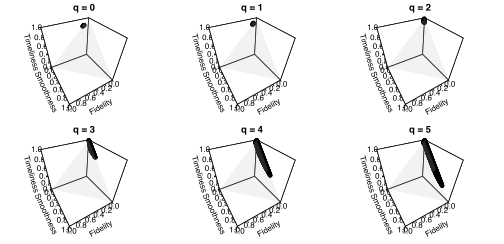
\includegraphics[height=0.6\paperheight]{img/lc6d0-1} \end{center}
\end{frame}

\hypertarget{comparaison-des-muxe9thodes}{%
\section{Comparaison des méthodes}\label{comparaison-des-muxe9thodes}}

\begin{frame}{Sommaire}
\protect\hypertarget{sommaire-1}{}
\tableofcontents[currentsection, hideothersubsections]
\end{frame}

\hypertarget{muxe9thodologie}{%
\subsection{Méthodologie}\label{muxe9thodologie}}

\begin{frame}[fragile]{Méthodologie}
\protect\hypertarget{muxe9thodologie-1}{}
2 404 séries CJO (\texttt{sts\_inpr\_m}, IPI de l'UE) :

\begin{enumerate}
\tightlist
\item
  Désaisonnalisation avec X-13ARIMA (\texttt{RJDemetra::x13}) à chaque
  date pour extraire : série linéarisée, longueur des filtres saisonnier
  et tendance, schéma de décomposition et I-C ratio
\end{enumerate}

\pause

\begin{enumerate}
\setcounter{enumi}{1}
\tightlist
\item
  Désaisonnalisation en \textbf{fixant} la série linéarisée et tous les
  autres paramètres et en utilisant un filtre spécifique pour la
  tendance-cycle (\texttt{rjdfilters::x11()})
\end{enumerate}

\pause

\begin{enumerate}
\setcounter{enumi}{2}
\item
  À chaque date, estimation des points de retournement :

  \begin{itemize}
  \item
    redressements : \(y_{t-3}\geq y_{t-2}\geq y_{t-1}<y_t\leq y_{t+1}\)
  \item
    ralentissements :
    \(y_{t-3}\leq y_{t-2}\leq y_{t-1}>y_t\geq y_{t+1}\)
  \end{itemize}
\end{enumerate}

\pause

Déphasage = temps nécessaire pour détecter le bon point de retournement
sans révision
\end{frame}

\hypertarget{un-exemple}{%
\subsection{Un exemple}\label{un-exemple}}

\begin{frame}{IPI fabrication de ciment, chaux et plâtre (C235) en
Allemagne (point de retournement en février 2020)}
\protect\hypertarget{ipi-fabrication-de-ciment-chaux-et-pluxe2tre-c235-en-allemagne-point-de-retournement-en-fuxe9vrier-2020}{}
\begin{center}\includegraphics[height=0.5\paperheight]{img/simulations/c235_de_x13} \end{center}
\end{frame}

\begin{frame}{}
\protect\hypertarget{section}{}
\begin{center}\includegraphics[height=0.5\paperheight]{img/simulations/c235_de_lc} \includegraphics[height=0.5\paperheight]{img/simulations/c235_de_ql} \end{center}
\end{frame}

\begin{frame}{}
\protect\hypertarget{section-1}{}
\begin{center}\includegraphics[height=0.5\paperheight]{img/simulations/c235_de_cq} \includegraphics[height=0.5\paperheight]{img/simulations/c235_de_daf} \end{center}
\end{frame}

\begin{frame}{}
\protect\hypertarget{section-2}{}
\begin{center}\includegraphics[height=0.5\paperheight]{img/simulations/c235_de_rkhs_timeliness} \includegraphics[height=0.5\paperheight]{img/simulations/c235_de_fst_lc} \end{center}
\end{frame}

\begin{frame}{}
\protect\hypertarget{section-3}{}
\begin{center}\includegraphics[height=0.5\paperheight]{img/simulations/c235_de_fst_lc_min} \includegraphics[height=0.5\paperheight]{img/simulations/c235_de_fst_lc_med} \end{center}
\end{frame}

\hypertarget{duxe9phasage}{%
\subsection{Déphasage}\label{duxe9phasage}}

\begin{frame}{Déphasage dans la détection de points de retournement en
2020}
\protect\hypertarget{duxe9phasage-dans-la-duxe9tection-de-points-de-retournement-en-2020}{}
Pour les séries dont le filtre symétrique utilisé pour la tendance-cycle
est de longueur 13 (771 séries)

\footnotesize

\alt<2>{\newcolumntype{C}{>{\columncolor{processblue!30}}c}}{\newcolumntype{C}{c}}

\alt<3>{\newcolumntype{D}{>{\columncolor{processblue!30}}c}}{\newcolumntype{D}{c}}

\alt<4>{\newcolumntype{E}{>{\columncolor{processblue!30}}c}}{\newcolumntype{E}{c}}

\begin{table}[!h]
\centering
\begin{tabular}[t]{lCCDDDEEEE}
\toprule
\multicolumn{7}{c}{ } & \multicolumn{3}{c}{\textbf<4>{FST - LC}} \\
\cmidrule(l{3pt}r{3pt}){8-10}
  & \textbf<2>{X-13ARIMA} & \textbf<2>{LC} & \textbf<3>{QL} & \textbf<3>{CQ} & \textbf<3>{DAF} & $b_{q,\varphi}$ & \textbf<4>{Min.} & \textbf<4>{Max.} & \textbf<4>{Méd.}\\
\midrule
Min & 2,0 & 2,0 & 2,0 & 2,0 & 2,0 & 2,0 & 2,0 & 2,0 & 2,0\\
Q1 & 3,0 & 4,0 & 3,0 & 2,0 & 2,0 & 6,0 & 6,0 & 6,0 & 6,0\\
Median & 4,0 & 4,0 & 4,0 & 6,0 & 6,0 & 6,0 & 7,0 & 6,0 & 6,0\\
Q3 & 5,0 & 5,0 & 7,0 & 7,0 & 7,0 & 7,0 & 7,0 & 6,0 & 7,0\\
Max & 14,0 & 14,0 & 14,0 & 14,0 & 14,0 & 14,0 & 14,0 & 14,0 & 14,0\\
\addlinespace
Mean & 4,5 & 4,7 & 5,1 & 5,4 & 5,5 & 6,6 & 7,0 & 6,5 & 6,6\\
\bottomrule
\end{tabular}
\end{table}
\end{frame}

\hypertarget{conclusion}{%
\section{Conclusion}\label{conclusion}}

\hypertarget{conclusion-1}{%
\subsection{Conclusion}\label{conclusion-1}}

\begin{frame}[fragile]{Conclusion}
\protect\hypertarget{conclusion-2}{}
\begin{itemize}
\tightlist
\item
  Dans la construction des filtres asymétriques, on peut se restreindre
  à ceux qui conserve les polynômes de degré au plus 1 (et exclure les
  filtres QL, CQ et DAF)
\end{itemize}

\bigskip

\pause

\begin{itemize}
\tightlist
\item
  Durant la crise du COVID-19, la méthode actuelle X-13ARIMA semble
  satisfaisante en moyenne\ldots{} \pause mais peut provenir des
  définitions, indicateurs et méthodologie utilisés
\end{itemize}

\bigskip

\pause

\begin{itemize}
\tightlist
\item
  Dans certains cas des filtres alternatifs peuvent aider
  \faIcon{arrow-circle-right} \texttt{rjdfilters} peut aider à comparer
  les résultats
\end{itemize}
\end{frame}

\begin{frame}{What next\bcquestion}
\protect\hypertarget{what-next}{}
\begin{itemize}
\tightlist
\item
  Comprendre quand et pourquoi une méthode est plus performante qu'une
  autre
\end{itemize}

\pause

\begin{itemize}
\tightlist
\item
  Etudes sur d'autres données avec d'autres méthodes
\end{itemize}

\pause

\begin{itemize}
\tightlist
\item
  Utiliser des paramètres différents en fin de période ?
\end{itemize}

\pause

\begin{itemize}
\tightlist
\item
  Impact des points atypiques ? quid des méthodes robustes ?
\end{itemize}
\end{frame}

\begin{frame}{Merci pour votre attention}
\protect\hypertarget{merci-pour-votre-attention}{}
Package \faIcon{r-project}{}:

\href{https://github.com/palatej/rjdfilters}{\faGithub{} palatej/rjdfilters}

\faIcon{desktop} Rapport en ligne :
\url{https://aqlt-stage3a.netlify.app/}
\end{frame}

\end{document}
